\chapter{Ejemplos de programas}
   \label{Ejemplos-Programas}

\section{Dibujar casas}
   \label{Dibujar-casas}

\noindent \texttt{para casa :c} 

\noindent \texttt{ repite 4 [}

  \texttt{avanza (20*:c) giraderecha 90 ]}

\noindent \texttt{ avanza (20*:c)}

\noindent \texttt{ giraderecha 30}

\noindent \texttt{ repite 3 [}

  \texttt{avanza (20*:c) giraderecha 120 ]}

\noindent \texttt{fin} \\

\noindent \texttt{para colocar :c}

\noindent \texttt{ subel\'apiz}

\noindent \texttt{ giraizquierda 30}

\noindent \texttt{ retrocede (:c*20)}

\noindent \texttt{ giraderecha 90}

\noindent \texttt{ avanza (:c*22)}

\noindent \texttt{ giraizquierda 90}

\noindent \texttt{ bajal\'apiz}

\noindent \texttt{fin} \\

\noindent \texttt{para casas}

\noindent \texttt{ borrapantalla}

\noindent \texttt{ ocultatortuga}

\noindent \texttt{ subel\'apiz}

\noindent \texttt{ giraizquierda 90}

\noindent \texttt{ avanza 200}

\noindent \texttt{ giraderecha 90}

\noindent \texttt{ bajal\'apiz}

\noindent \texttt{ repitepara [n 3 7 2]}

\texttt{[ casa :n colocar :n ]}

\noindent \texttt{ casa 10}

\noindent \texttt{fin}
\begin{center}
   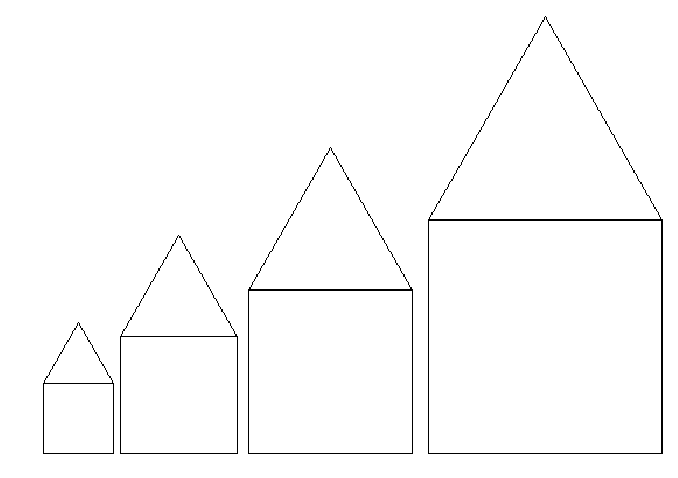
\includegraphics[scale=0.4]{Imagenes/13_Ejemplos/casas.png}
\end{center}

\section{Dibujar un rect\'angulo s\'olido}
   \label{Dib-Rectangulo-Solido}

\begin{verbatim}
   para rect :alto :largo
    si :alto = 0 | :largo = 0 [alto]
    repite 2 [
       avanza :alto
       giraderecha 90
       avanza :largo
       giraderecha 90 ]
    rect :alto -1 :largo -1
   fin \end{verbatim}
\begin{center}
   
\includegraphics[scale=0.6]{Imagenes/13_Ejemplos/rectangulo.png}
\end{center}

\section{Factorial}
   \label{Factorial}
   \index{Factorial}

Recordatorio: \texttt{5! = 5 * 4 * 3 * 2 * 1}
\begin{verbatim}
   para factorial :n 
     si :n = 1 
      [devuelve 1]
      [devuelve :n * factorial (:n - 1)]
   fin \end{verbatim}
\begin{quote}
   \noindent \textbf{Ejemplo}:
   \begin{verbatim}
      escribe factorial 5 --> 120.0
      escribe factorial 6 --> 720.0 \end{verbatim}
\end{quote}

\section{Copo de nieve (Gracias a Georges No\"el)}
   \label{Copo-de-nieve}
   \index{Copo de nieve}

\begin{verbatim}
   para copo :orden :lar
     si (:orden < 1) | (:lar < 1)
      [av :lar alto]
     copo :orden-1 :lar/3
     giraizquierda 60
     copo :orden-1 :lar/3
     giraderecha 120
     copo :orden-1 :lar/3
     giraizquierda 60
     copo :orden-1 :lar/3
   fin

   para coponieve :orden :lar 
     repite 3 [
       giraderecha 120 
       copo :orden :lar ]
   fin \end{verbatim}
Ej: \texttt{coponieve 5 450} 
\begin{center}
   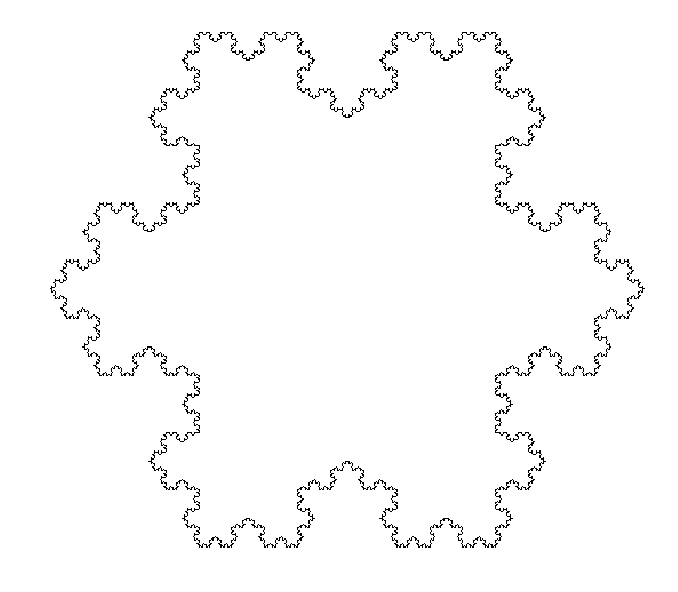
\includegraphics[scale=0.4]{Imagenes/13_Ejemplos/CopoNieve.png}
\end{center}

\section{Escritura}
   \label{Escritura}

\begin{verbatim}
   para escribir 
     ocultatortuga
     repite 40 [
       avanza 30
       giraderecha 9
       poncolorlapiz azar 7
       rotula [XLogo es genial!] ] 
   fin \end{verbatim}
\begin{center}
   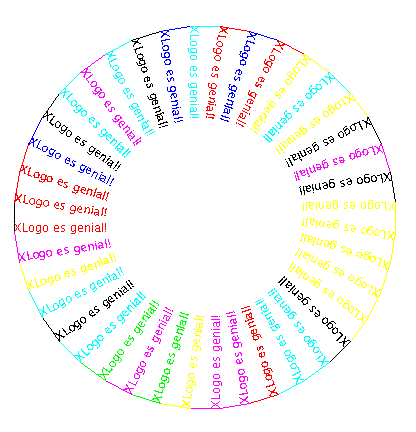
\includegraphics[scale=0.6]{Imagenes/13_Ejemplos/Escritura.png}
\end{center}

\section{Conjugaci\'on (s\'olo verbos regulares)}
   \label{Conjugacion}

\subsection{Primera versi\'on}
\begin{quote}
   \verb+para futuro :verbo+ \\
   \verb+  es frase "yo palabra :verbo "+\texttt{\'e}\\
   \verb+  es frase "t+\texttt{\'u}\verb+ palabra :verbo "+\texttt{\'as}\\
   \verb+  es frase "+\texttt{\'el}\verb+ palabra :verbo "+\texttt{\'a}\\
   \verb+  es frase "nosotros palabra :verbo "emos+\\
   \verb+  es frase "vosotros palabra :verbo "+\texttt{\'eis}\\
   \verb+  es frase "ellos palabra :verbo "+\texttt{\'an}\\
   \verb+fin+\end{quote}
\begin{quote}
   \noindent \textbf{Ejemplo}: \verb+futuro "amar+

   \texttt{yo amar\'e}\\
   \texttt{t\'u amar\'as}\\
   \texttt{\'el amar\'a}\\
   \texttt{nosotros amaremos}\\
   \texttt{vosotros amar\'eis}\\
   \texttt{ellos amar\'an}
\end{quote}

\subsection{Segunda versi\'on}

\begin{quote}
   \verb+para futuro :verbo+\\
   \verb+  haz "pronombres [yo +\texttt{t\'u \'el nosotros vosotros ellos]}\\
   \verb+  haz "terminaciones [+\texttt{\'e \'as \'a emos \'eis \'an]}\\
   \verb+  repitepara [i 1 6]+\\
   \verb+   [ es fr elemento :i :pronombres palabra :verbo elemento :i :terminaciones ]+\\
   \verb+fin+ \end{quote}
\begin{quote}
   \noindent \textbf{Ejemplo}: \verb+futuro "amar+

   \texttt{yo amar\'e}\\
   \texttt{t\'u amar\'as}\\
   \texttt{\'el amar\'a}\\
   \texttt{nosotros amaremos}\\
   \texttt{vosotros amar\'eis}\\
   \texttt{ellos amar\'an}
\end{quote}

\subsection{Tercera versi\'on (con recurrencia)}

\begin{quote}
   \verb+para futuro :verbo +\\
   \verb+  haz "pronombres [yo +\texttt{t\'u \'el nosotros vosotros ellos]}\\
   \verb+  haz "terminaciones [+\texttt{\'e \'as \'a emos \'eis \'an]}\\
   \verb+  conjugar :verbo :pronombres :terminaciones+\\
   \verb+fin+\\

   \verb+para conjugar :verbo :pronombres :terminaciones+\\
   \verb+  si vacio? :pronombres [alto]+\\
   \verb+  es fr primero :pronombres palabra :verbo primero :terminaciones+\\
   \verb+  conjugar :verbo mp :pronombres mp :terminaciones+\\
   \verb+fin+ \end{quote}
\begin{quote}
   \noindent \textbf{Ejemplo}: \verb+futuro "amar+

   \texttt{yo amar\'e}\\
   \texttt{t\'u amar\'as}\\
   \texttt{\'el amar\'a}\\
   \texttt{nosotros amaremos}\\
   \texttt{vosotros amar\'eis}\\
   \texttt{ellos amar\'an}
\end{quote}

\section{Colores}
   \label{EjColores}
   \index{Colores (ejemplo)}

\subsection{Introducci\'on}
   \label{Colores-Introduccion}

Primero, algunas aclaraciones: Habr\'as visto en la secci\'on
\ref{AcercaColores} que el comando \texttt{poncl} puede tomar como
argumento tanto un n\'umero como una lista. Aqu\'i nos
centraremos en codificar valores RVA. Cada color en \textsc{XLogo}
est\'a codificado usando tres valores: rojo, verde y azul, de ah\'i RVA
(RGB en ingl\'es). 

Estos tres n\'umeros conforman una lista que es argumento de la primitiva
\texttt{poncl}, por lo que representan respectivamente los componentes
rojo, verde y azul de un color. Esta manera de codificar no es muy
intuitiva, as\'i que para tener una idea del color que obtendr\'as puedes
usar la caja de di\'alogo \textbf{Herramientas $\rightarrow$ Elegir color del l\'apiz}.

Sin embargo, usando esta forma de codificar colores, se hace muy f\'acil
transformar una imagen. Por ejemplo, si quieres convertir una foto color
en escala de grises, puedes cambiar cada punto (p\'ixel) de la imagen a un
valor promedio de los 3 componentes RVA. Imagina que el color de un punto
de la imagen est\'a dado por \texttt{[0 100 80]}. Calculamos el
promedio: \texttt{(0 + 100 + 80)/3 = 60}, y asignamos el color
\texttt{[60~60~60]} a este punto. Esta operaci\'on debe ser realizada para
cada punto de la imagen.

\subsection{Pr\'actica: Escala de grises}
   \label{Colores-Practica}

Vamos a transformar una imagen color de 100 por 100 a escala de
grises. Esto significa que tenemos \texttt{100 * 100 = 10000} puntos a
modificar.

La imagen de ejemplo utilizada aqu\'i est\'a disponible en la siguiente
direcci\'on:
\begin{verbatim}
   http://xlogo.tuxfamily.org/images/transfo.png \end{verbatim}
As\'i es como vamos a proceder: primero, nos referiremos al punto superior
izquierdo como \texttt{[0~0]}. Luego, la tortuga examinar\'a los
primeros 100 puntos (pixeles) de la primera l\'inea, seguidos por los
primeros 100 de la segunda, y as\'i sucesivamente. Cada vez tomaremos
el color del punto usando \texttt{encuentracolor}, y el color ser\'a cambiado
por el promedio de los tres \texttt{[r~v~a]} valores. Aqu\'i est\'a
el c\'odigo principal: (No olvides cambiar la ruta del archivo en el
procedimiento!)

\begin{verbatim}
para transform
# Debes cambiar la ruta de la imagen transfo.png
# Ej: cargaimagen [/home/usuario/imagenes/transfo.png]
  borrapantalla ocultatortuga
  pondirectorio "/home/usuario/imagenes
  cargaimagen "transfo.png
  escalagris
fin

para escalagris
  repitepara [y 0 -100 -1]
    [ repitepara [x 0 100]
# asignamos el promedio de color del punto al color del lapiz
      [ poncolorlapiz pixel encuentracolor lista :x :y
# convertimos el punto escala de grises 
        punto lista :x :y ] ]
fin

para pixel :lista1
# devuelve el promedio de los 3 numeros [r v a]
  haz "r primero :lista1 
  haz "lista1 menosprimero :lista1 
  haz "v primero :lista1 
  haz "lista1 menosprimero :lista1 
  haz "a primero :lista1 
  haz "color redondea (:r+:v+:a)/3
  devuelve frase :color frase :color :color 
fin \end{verbatim}
\begin{center}
  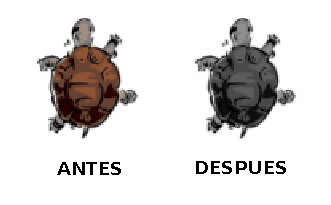
\includegraphics[scale=0.6]{Imagenes/13_Ejemplos/colores1.png}
\end{center}

\subsection{Negativo}
   \label{Colores-Negativo}

Para cambiar una imagen a su negativo, se puede usar el mismo proceso
de la escala de grises, excepto que en lugar de hacer el promedio
de los n\'umeros \texttt{[r~v~a]}, los reemplazamos por su complemento,
o sea la diferencia a 255. 

\noindent \textbf{Ejemplo}: Si un punto (p\'ixel) tiene un color
\texttt{[2~100~200]}, lo reemplazamos con \texttt{[253~155~55]}.
Podr\'iamos usar el mismo c\'odigo que en el ejemplo anterior,
cambiando \'unicamente el procedimiento \texttt{pixel}, pero veamos
un procedimiento recursivo:
\begin{verbatim}
para transform2
# Debes cambiar la ruta de la imagen transfo.png
# Ej: c:\Mis Documentos\Mis imagenes\transfo.png
  borrapantalla
  ocultatortuga
  pondirectorio "c:\\Mis\ Documentos\\Mis\ imagenes
  cargaimagen "transfo.png
  negativo 0 0
fin

para negativo :x :y
  si :y = -100
   [ alto ]
   [ si :x = 100
     [ haz "x 0 haz "y :y-1]
     [ poncolorlapiz pixel2 encuentracolor lista :x :y
       punto lista :x :y ] ] 
  negativo :x+1 :y
fin

para pixel2 :lista1
# devuelve el promedio de los 3 numeros [r v a]
  haz "r primero :lista1 
  haz "lista1 menosprimero :lista1 
  haz "v primero :lista1 
  haz "lista1 menosprimero :lista1 
  haz "a primero :lista1 
  devuelve frase (255 - :r) frase (255 - :v) (255 - :a)
fin \end{verbatim}
\begin{center}
   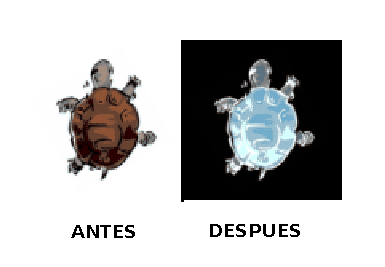
\includegraphics[scale=0.6]{Imagenes/13_Ejemplos/colores2.png}
\end{center}

\section{Listas (Gracias a Olivier SC)}
   \index{Listas}
   \label{Ejemplo-Listas}

Supongo que apreciar\'as este hermoso programa:
\begin{verbatim}
   para revertir :w 
     si vacio? :w
       [devuelve "]
       [devuelve palabra ultimo :w revertir menosultimo :w ]
   fin

   para palindromo :w
    si :w = revertir :w
      [devuelve "cierto]
      [devuelve "falso]
   fin

   para palin :n
     si palindromo :n
      [escribe :n alto]
      [haz "texto suma :n revertir :n
       haz "texto frase "igual\ a :texto
       haz "texto frase revertir :n :texto
       haz "texto frase "mas :texto
       haz "texto frase :n :texto
       escribe :texto
       palin :n + revertir :n ]
   fin \end{verbatim}
\begin{quote}
   \noindent \textbf{Ejemplo}: \texttt{palin 78}
   \begin{verbatim}
      78 mas 87 igual a 165
      165 mas 561 igual a 726
      726 mas 627 igual a 1353
      1353 mas 3531 igual a 4884
      4884 \end{verbatim}
\end{quote}

\section{Un lindo medall\'on}
   \index{Medall\'on}
   \label{Medallon}
\begin{verbatim}
   para roset
     pongrosor 2
     repite 6 [
       repite 60
        [avanza 2 giraderecha 1]
       giraderecha 60
       repite 120
        [avanza 2 giraderecha]
       giraderecha 60 ]
     pongrosor 1
   fin

   para roseton 
     roset 
     repite 30
       [avanza 2 giraderecha 1]
     roset 
     repite 15
       [avanza 2 giraderecha 1]
     roset
     repite 30
       [avanza 2 giraderecha 1]
     roset
   fin \end{verbatim}

\textbf{Ejemplo}: 
\begin{verbatim}
   borrapantalla ocultatortuga
   poncolorpapel 0 poncolorlapiz 5
   roset
   subelapiz ponposicion [-300 0] bajalapiz
   ponrumbo 0 roseton \end{verbatim}
\begin{center}
   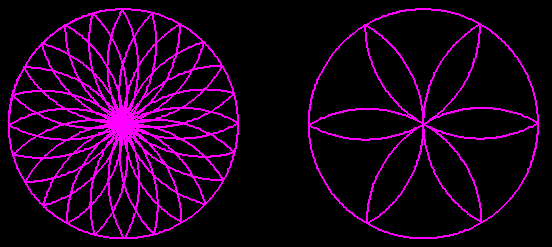
\includegraphics[width=10cm]{Imagenes/13_Ejemplos/roseton.png}
\end{center}